%% =====================================================================
%% Probing-Resistant Masked Hardware
%% Target venue: IEEE Transactions on Information Forensics and Security (TIFS)
%% IEEEtran journal class. Compile with pdflatex (x2) + bibtex if using .bib.
%% Placeholders marked with TODO must be completed before submission.
%% =====================================================================
\documentclass[lettersize,journal]{IEEEtran}
\usepackage{amsmath,amsfonts,amssymb}
\usepackage{amsthm}
\usepackage{algorithm}
\usepackage{algorithmic}
\usepackage{array}
\usepackage{booktabs}
\usepackage[caption=false,font=normalsize,labelfont=sf,textfont=sf]{subfig}
\usepackage{textcomp}
\usepackage{stfloats}
\usepackage{url}
\usepackage{graphicx}
\usepackage{cite}
\usepackage{tikz}
\usetikzlibrary{arrows.meta,positioning,shapes.geometric,fit,backgrounds}
\hyphenation{op-tical net-works semi-conduc-tor IEEE-Xplore}

%% Theorem-like environments
\newtheorem{theorem}{Theorem}
\newtheorem{lemma}{Lemma}
\newtheorem{definition}{Definition}
\newtheorem{corollary}{Corollary}

%% Convenience macros
\newcommand{\GF}{\mathrm{GF}}
\newcommand{\share}[2]{#1^{(#2)}}
\newcommand{\Adv}{\mathcal{A}}
\newcommand{\prob}[1]{\Pr\!\left[#1\right]}

\begin{document}

\title{Probing-Resistant Masked Hardware: Formal Security Proofs and Simulation-Based Side-Channel Verification}

\author{Anonymous Author(s)
\thanks{Manuscript under review, October 2026.
Author identities and affiliations are withheld for review.}
}

\markboth{IEEE Transactions on Information Forensics and Security,~Vol.~XX, No.~X, 2026}%
{Author \MakeLowercase{\textit{et al.}}: Probing-Resistant Masked Hardware}

\maketitle

\begin{abstract}
Masking is the prevailing algorithmic countermeasure against power and
electromagnetic side-channel analysis of cryptographic hardware, yet a
persistent gap remains between the abstract security order claimed by a
masking scheme and the leakage observed once physical effects such as
glitches and transitions are taken into account.
Our central contribution is to \emph{characterize} this
soundness gap in equipment-free evaluation: a value-based statistical
verifier can accept a design that a glitch-extended probe deterministically
breaks. The model-level distinction between value-based and
glitch-extended probes is classical~\cite{faust2018composable};
what has been missing is a characterization of \emph{when}
the cheaper channel's verdict is sound. We give such a
characterization via a cone-non-completeness condition on
register-input cones, prove that passing the corresponding
sound-by-construction lint forces the value-based and glitch-extended
verdicts to coincide, and exhibit an explicit first-order
witness that satisfies the value-based verifier while a
single robust probe recombines the secret. We implement the check on the
flattened gate-level netlist (seconds of run time): it accepts the final
first-order design, flags every cone that a gate-level statistical test shows
to leak in an earlier variant without operand refresh, and rejects controlled
violations (mask removal, register collapse).
We pair this static channel with a masked hardware construction whose
multiplication gadget is proven robust $d$-NI (for arbitrary $d$) via a
perfect-simulation argument. On the first-order AES S-box built from it,
PROLEAD reports $0$ leaking probing sets out of $14{,}400$ at $512{,}000$
simulations, while gate-level power simulation with TVLA reports no
detection; the TVLA/MI channel has low detection power on its
Hamming-distance traces, so we treat it as supporting evidence only. The
design uses $56$ fresh-random bits per invocation and a $17$-cycle
latency, i.e.\ more randomness and latency than DOM or HPC2 S-boxes; we do
not claim a cost advantage. Empirical evaluation is limited to $d{=}1$.
Together these results connect a provable gadget-level guarantee with
reproducible, equipment-free verification at first order.
\end{abstract}

\begin{IEEEkeywords}
Side-channel analysis, masking, threshold implementation, probing security,
formal verification, TVLA, hardware security, cryptographic hardware.
\end{IEEEkeywords}

\section{Introduction}
\IEEEPARstart{C}{ryptographic} hardware such as AES accelerators can leak secret
key material through physical side channels: an adversary who measures the
instantaneous power consumption or electromagnetic (EM) emanations of a device
during encryption can recover the key using differential or correlation power
analysis (DPA/CPA)~\cite{kocher1999dpa,brier2004cpa}. \emph{Masking} is the
most widely deployed algorithmic countermeasure: every secret-dependent value
$x$ is split into $d+1$ random shares $\share{x}{0},\dots,\share{x}{d}$ such
that any $d$ of them are jointly independent of $x$, forcing the attacker to
combine $d+1$ leakage points and thereby raising the measurement cost
exponentially in the noise level~\cite{ishai2003private,chari1999towards}.

Despite two decades of progress, a fundamental gap persists between the
\emph{claimed} security order of a masking scheme and the leakage \emph{actually
observed} in silicon. The root cause is that physical hardware violates the
idealized assumptions of the abstract model: combinational glitches and signal
transitions recombine shares within a single clock cycle, degrading a nominally
$d$-th order secure design to a lower effective order~\cite{mangard2005glitch,
nikova2006threshold}. Threshold Implementations (TI) and their successors
(DOM, HPC) address glitches through non-completeness and register
barriers~\cite{nikova2006threshold,gross2016dom,cassiers2020hpc}, but verifying
that a concrete netlist attains its intended order remains error-prone.

\textbf{Our approach.} We argue that the probing-security theory developed for
secure multiparty computation (MPC)~\cite{ishai2003private} provides exactly the
right abstraction to close this gap when it is (a) lifted to the
glitch-extended hardware model and (b) paired with reproducible simulation-based
verification. Building on this observation, we design a masked hardware
construction and prove its security in the robust $d$-probing
model~\cite{faust2018composable}, then check the first-order instance with equipment-free,
simulation-based tools.

\textbf{Contributions.} This paper makes the following contributions:
\begin{itemize}
  \item We characterize the \emph{soundness gap} between equipment-free
        value-based statistical verification and glitch-extended probing,
        and give a sound-by-construction cone-non-completeness lint that
        closes it at first order: passing the lint certifies that the two verdicts
        coincide at first order, and failing it exhibits a concrete recombination witness
        (Section~\ref{sec:soundness}, Definition~\ref{def:cone-nc},
        Theorems~\ref{thm:lint-sound} and~\ref{thm:gap-witness},
        Corollary~\ref{cor:lint}).
  \item We back the gap-witness theorem with a fully worked constructive
        artifact in the Supplemental Material: an algebraic derivation of the
        first-order witness, a cone that deterministically recombines the
        secret under a glitch-extended probe while its registered value
        remains uniform and independent of the secret, establishing the
        concrete gap of
        Theorem~\ref{thm:gap-witness} (Supplemental Material, Section~S2).
  \item We implement the lint on the flattened synthesized netlist
        ($67{,}344$ combinational gates, $818$ flip-flops; run time in
        seconds) and cross-check it against a gate-level statistical test
        on the final design, on an earlier variant without operand refresh,
        and on two controlled violations
        (Table~\ref{tab:lint-ablation}, Fig.~\ref{fig:cone-gap}).
  \item We give sufficient conditions under which our masked gate construction
        attains order-$d$ security in the robust (glitch-extended) probing
        model, and prove them formally (Section~\ref{sec:security}).
  \item We provide a simulation-based verification methodology combining the
        formal tool PROLEAD with gate-level power simulation and TVLA, and
        report that, at first order, the observed results are consistent with
        the proven order (Sections~\ref{sec:method}--\ref{sec:eval}); together with
        the static lint above, this yields three equipment-free
        verification channels on the same netlist, whose differing
        detection powers we characterize explicitly rather than treat as
        interchangeable.
  \item On protected AES S-box benchmarks we compare against TI, DOM, and
        HPC on fresh randomness and latency, and report that our construction
        is more expensive on both
        (Table~\ref{tab:cost}, Section~\ref{sec:eval}).
\end{itemize}

The remainder of the paper is organized as follows.
Section~\ref{sec:background} reviews masking and probing models.
Section~\ref{sec:model} states the threat model and security definitions.
Section~\ref{sec:construction} presents our construction.
Section~\ref{sec:security} contains the formal security analysis.
Sections~\ref{sec:method} and~\ref{sec:eval} describe the verification
methodology and experimental results. Section~\ref{sec:related} surveys related
work, and Section~\ref{sec:conclusion} concludes.

\section{Background and Preliminaries}
\label{sec:background}

\subsection{Boolean Masking}
Let $x \in \GF(2^n)$ be a sensitive value. A $(d{+}1)$-sharing of $x$ is a tuple
$(\share{x}{0},\dots,\share{x}{d})$ with
$x = \bigoplus_{i=0}^{d}\share{x}{i}$, where $\share{x}{0},\dots,\share{x}{d-1}$
are drawn uniformly at random and $\share{x}{d}$ is chosen to satisfy the
invariant. Linear functions are applied share-wise; the difficulty lies in
securely evaluating non-linear operations (e.g., the AES S-box multiplicative
inverse in $\GF(2^8)$).

\subsection{Threshold Implementations and Successors}
Threshold Implementations~\cite{nikova2006threshold} enforce three properties
---correctness, non-completeness, and uniformity---so that no combinational
function depends on all shares of any secret, which provides provable
first-order security even in the presence of glitches. Domain-Oriented Masking
(DOM)~\cite{gross2016dom} and Hardware Private Circuits
(HPC)~\cite{cassiers2020hpc} generalize this to arbitrary orders while reducing
fresh randomness and enabling composability.

\subsection{Probing Models}
In the $d$-probing model~\cite{ishai2003private}, an adversary places up to $d$
probes on internal wires and learns their exact values; a circuit is secure if
any such set of $d$ probes is independent of the secret. The
\emph{glitch-extended} (robust) probing model~\cite{faust2018composable}
accounts for combinational recombination by letting a single probe on a wire
reveal all stable inputs to the combinational cone feeding it since the last
register stage. We adopt the robust model throughout.

\subsection{Relation to Prior Verification Frameworks}
\label{sec:prior-verifiers}

Several tools already establish or check probing security for masked
hardware. We briefly contrast them with the sound-lint proposed in
\S\ref{sec:soundness} to make the contribution of this paper precise.

\paragraph{SILVER~\cite{knichel2020silver} and exact verifiers.} SILVER
performs an exact, BDD-based analysis of glitch-extended probes on a
gate-level netlist and issues a definitive verdict for the given
design; exact procedures of this kind are costly on large netlists, which
is why full-S-box and full-round designs are usually checked with
composition arguments or statistical tools. Bloem \emph{et
al.}~\cite{bloem2018formal} established the probing security of masked
hardware in the presence of glitches by exact formal verification, and
Shahmirzadi \emph{et al.}~\cite{shahmirzadi2021records} verified
first-order masked AES implementations with SILVER. MaskVerif~\cite{maskverif2015}
and IronMask~\cite{ironmask2022} decide probing-style security
properties of masked implementations, and VERICA~\cite{verica2022}
targets combined leakage-and-fault attacks. All of these decide
properties of the circuit model itself; none exposes an intermediate
abstraction whose verdict can be certified sound with respect to a
statistical leakage bound, so their outputs cannot be composed with a
DDF14-style noisy-leakage argument without re-running the underlying
decision procedure.

\paragraph{PROLEAD~\cite{muller2022prolead}.} PROLEAD is
simulation-based: it enumerates glitch-extended probe sets up to a
fixed order and runs statistical tests over sampled traces. PROLEAD
is highly precise on the traces it observes and is our
gold-standard cross-check throughout \S\ref{sec:results}. Its
guarantees, however, are asymptotic in the number of simulations
and offer no completeness certificate: a probe set that is not
sampled cannot be ruled leaky, and a scheme that passes at
$5\times10^{5}$ simulations may fail at $10^{7}$. PROLEAD therefore
answers ``does this design appear secure under the simulation
budget?'' rather than ``is every probe cone provably non-leaking?''

\paragraph{HPC2 / PINI~\cite{cassiers2020hpc,cassiers2021tight}.}
HPC2 and the broader PINI methodology are compositional
frameworks: they provide gadget-level primitives whose composition
is guaranteed to remain secure. They are constructive rather than
diagnostic---once a design is expressed as a composition of PINI
gadgets, security follows by inspection---but they do not verify
arbitrary post-synthesis netlists such as those emitted by Yosys
optimization passes, where original gadget boundaries are erased.

\paragraph{Cardinal and algebraic
composition~\cite{belaid2025cardinal,jahandideh2024algebraic}.}
Recent algebraic verifiers such as Cardinal and its precursors
target random-probing composition and achieve strong asymptotic
bounds under the assumption of noisy wires. Their verdicts are
essentially algebraic; the required per-wire noise threshold is
not directly measured from the target netlist but stipulated as an
assumption. Our robust-probing claims are
complementary: they are checked on the netlist itself and make no
assumption on the measurement noise.

\paragraph{This work: sound-lint as a certified pre-filter.}
Positioned at a strictly lower cost than SILVER and PROLEAD
---linear-time union-find on the flattened netlist
(\S\ref{sec:lint-eval}, seconds on $67{,}344$ gates)---our lint
does not attempt to be a decision procedure for probing security.
Instead, Theorem~\ref{thm:lint-sound} proves that a PASS verdict
rules out an entire structural class of first-order leakage
(co-share appearance in a common glitch cone), and
Theorem~\ref{thm:gap-witness} exhibits an equivalence-preserving
netlist perturbation on which SILVER and PROLEAD agree but no
purely combinational lint can. The lint is therefore a
soundness-certified pre-filter that complements the exact but
heavier tools rather than replacing them, and its cross-check against a
statistical test (Table~\ref{tab:lint-ablation}) empirically supports this
positioning.

\section{Threat Model and Security Definitions}
\label{sec:model}
We consider an adversary $\Adv$ who obtains noisy observations of the power/EM
leakage of a masked hardware implementation during operation on a fixed but
unknown key. $\Adv$ may choose plaintexts adaptively and collect an
unbounded number of traces. We abstract physical leakage by the robust
$d$-probing model and require security in the following sense.

\begin{definition}[Robust $d$-probing security]
\label{def:probing}
A masked circuit $C$ is \emph{robust $d$-probing secure} if, for every set
$\mathcal{P}$ of at most $d$ glitch-extended probes, the joint distribution of
the probed values is independent of the secret $x$; equivalently, the mutual
information $I(x;\mathcal{P}) = 0$.
\end{definition}

\begin{definition}[Composability]
\label{def:comp}
A gadget is $d$-Non-Interfering (NI) if any $d$ probes can be simulated using at
most $d$ of its input shares, and $d$-Strong-Non-Interfering (SNI) if the
simulation additionally separates internal and output probes. SNI gadgets
compose to yield larger $d$-probing secure circuits~\cite{barthe2016strong}.
\end{definition}

\section{Proposed Masking Construction}
\label{sec:construction}
We target the non-linear core of the AES S-box, i.e., the multiplicative inverse
in $\GF(2^8)$, computed with the Itoh--Tsujii addition chain
$x^{-1}=x^{254}$: a chain of share-wise Frobenius squarings
($x^{2},x^{4},\dots,x^{128}$) interleaved with six field multiplications
($x^{2}{\cdot}x^{4}$, $x^{6}{\cdot}x^{8}$, $x^{14}{\cdot}x^{16}$,
$x^{30}{\cdot}x^{32}$, $x^{62}{\cdot}x^{64}$, $x^{126}{\cdot}x^{128}$).
Linear layers (squarings and the final AES affine map) are shared
component-wise; the multiplier is the only gadget requiring fresh
randomness, apart from one operand refresh detailed below.

Our multiplier gadget builds on the domain-oriented masking (DOM)
multiplier~\cite{gross2016dom}. The two secret inputs $a,b\in\GF(2^m)$ are given
as independent $(d{+}1)$-sharings $(\share{a}{i})_{i}$ and $(\share{b}{j})_{j}$,
with each share assigned to its own \emph{domain}. The gadget produces a
$(d{+}1)$-sharing $(\share{c}{k})_{k}$ of $c=a\cdot b$ in three stages:
(i) all domain products $p_{ij}=\share{a}{i}\cdot\share{b}{j}$;
(ii) a \emph{cross-domain refresh} in which each unordered pair $\{i,j\}$ with
$i\neq j$ draws a single fresh mask $r_{ij}=r_{ji}$ that is added to both
$p_{ij}$ and $p_{ji}$; and (iii) a \emph{register barrier} that stores every
refreshed term before the domain compression $\share{c}{i}=\bigoplus_j q_{ij}$.
Sharing one mask across the symmetric pair guarantees correctness (the masks
cancel in $\bigoplus_i\share{c}{i}$), while the register barrier blocks glitch
propagation across domains. Algorithm~\ref{alg:mult} states the order-$d$ gadget
precisely; it consumes $R(d)=\binom{d+1}{2}$ fresh $m$-bit mask words ($m{=}8$ here) per multiplication.

\paragraph{Operand independence in the Itoh--Tsujii chain.}
The independence precondition on the multiplicand sharings is \emph{not}
automatic in the addition chain.  Squaring is $\mathbb{F}_2$-linear, so it
is applied share-wise, and the sharings of $x^{2^i}$ and $x^{2^j}$ produced
by the chain remain \emph{aligned} with the input sharing:
$\share{(x^{2^k})}{i}=\bigl(\share{x}{i}\bigr)^{\,2^k}$.  Feeding two such aligned
sharings directly into Algorithm~\ref{alg:mult} breaks the gadget's
precondition: a glitch-extended probe on the cross-term cone of the first
multiplication ($x^{2}{\cdot}x^{4}$) observes
$\{\share{(x^{2})}{0},\share{(x^{4})}{1}\}$, from which
$(\share{x}{0})^{\,4}\oplus(\share{x}{1})^{\,4}=(\share{x}{0}\oplus
\share{x}{1})^{4}=x^{4}$ is recombined \emph{deterministically} by one
offline squaring.  We therefore insert a single registered refresh on one operand of the first
multiplication,
$\share{(x^{4})'}{i}\leftarrow\mathrm{Reg}(\share{(x^{4})}{i}\oplus r_6)$,
where one fresh byte $r_6\in\GF(2^8)$ is added to both shares, $i\in\{0,1\}$
(the mask cancels in $\bigoplus_i\share{(x^{4})'}{i}$, so correctness is
preserved). Its role is blinding, not joint re-randomization: each refreshed
operand register is a blinded value in the sense of
Definition~\ref{def:cone-nc}, so every cross-term cone of the first
multiplication carries at most one unblinded share index, and the
recombination of Theorem~\ref{thm:gap-witness} is masked by the fresh pad.
Because the refresh does not decorrelate the two multiplicand sharings
jointly, the netlist-level claim is made through cone non-completeness
(Corollary~\ref{cor:comp}, Theorem~\ref{thm:lint-sound}), which the
implemented netlist passes.
In every later multiplication one operand is the previous multiplier's
output, already re-masked by that stage's $r_{01}$; every cross-term cone of
the next stage then pairs a blinded prior output with a single chain share,
which preserves cone non-completeness.  The first-order S-box thus consumes
$6$ refresh bytes $r_{01}$ (one per multiplication) plus $1$ operand-refresh
byte, i.e.\ $56$ fresh-random bits per invocation in total.

\begin{algorithm}[t]
\caption{Proposed order-$d$ masked multiplier}
\label{alg:mult}
\begin{algorithmic}[1]
\STATE \textbf{Input:} independent sharings $(\share{a}{i})_{i=0}^{d}$, $(\share{b}{j})_{j=0}^{d}$
\STATE \textbf{Output:} sharing $(\share{c}{k})_{k=0}^{d}$ with $c = a \cdot b$
\STATE sample fresh $r_{ij}\in\GF(2^m)$ for all $0\le i<j\le d$; set $r_{ji}\leftarrow r_{ij}$
\FOR{$i = 0$ \TO $d$}
  \FOR{$j = 0$ \TO $d$}
    \STATE $p_{ij} \leftarrow \share{a}{i} \cdot \share{b}{j}$ \COMMENT{domain product}
    \IF{$i = j$}
      \STATE $q_{ij} \leftarrow \mathrm{Reg}(p_{ij})$
    \ELSE
      \STATE $q_{ij} \leftarrow \mathrm{Reg}(p_{ij} \oplus r_{ij})$ \COMMENT{refresh + barrier}
    \ENDIF
  \ENDFOR
\ENDFOR
\FOR{$i = 0$ \TO $d$}
  \STATE $\share{c}{i} \leftarrow \bigoplus_{j=0}^{d} q_{ij}$ \COMMENT{domain compression}
\ENDFOR
\RETURN $(\share{c}{k})_{k=0}^{d}$
\end{algorithmic}
\end{algorithm}

\section{Formal Security Analysis}
\label{sec:security}
We establish, in order, correctness, output uniformity, glitch-robust
non-completeness, robust $d$-NI security with perfect simulation, first-order composition
through cone non-completeness, and the cost characterization. Throughout, $\mathrm{Reg}(\cdot)$ denotes
a synchronous register, and every combinational cone is delimited by the
register barrier of Algorithm~\ref{alg:mult}.

\begin{lemma}[Correctness]
\label{lem:correct}
The output of Algorithm~\ref{alg:mult} satisfies
$\bigoplus_{i=0}^{d}\share{c}{i}=a\cdot b$.
\end{lemma}
\begin{proof}
By construction,
$\bigoplus_i\share{c}{i}=\bigoplus_{i}\bigoplus_{j}q_{ij}
=\bigoplus_{i,j}p_{ij}\;\oplus\;\bigoplus_{i\neq j}r_{ij}$.
Each unordered pair $\{i,j\}$ contributes $r_{ij}=r_{ji}$ exactly twice, once in
$q_{ij}$ and once in $q_{ji}$, so $\bigoplus_{i\neq j}r_{ij}=0$. Hence
$\bigoplus_i\share{c}{i}=\bigoplus_{i,j}\share{a}{i}\share{b}{j}
=\big(\bigoplus_i\share{a}{i}\big)\big(\bigoplus_j\share{b}{j}\big)=a\cdot b$.
\end{proof}

\begin{lemma}[Output uniformity]
\label{lem:unif}
If the input sharings are uniform and independent, then every $d$ of the output
shares $(\share{c}{i})_{i=0}^{d}$ are jointly uniform and independent of $c$.
\end{lemma}
\begin{proof}
Fix any $d$ output shares, i.e., all but $\share{c}{k}$. For each $i\neq k$ the
term $q_{ik}=\mathrm{Reg}(\share{a}{i}\share{b}{k}\oplus r_{ik})$ carries the
fresh mask $r_{ik}=r_{ki}$, which occurs in $\share{c}{i}$ and, among all output
shares, only additionally in the excluded $\share{c}{k}$. Thus the $d$ masks
$\{r_{ik}\}_{i\neq k}$ are mutually independent and uniform, each appearing in
exactly one retained share. Conditioned on all remaining quantities, the map
from $(r_{ik})_{i\neq k}$ to the $d$ retained shares is a bijection, so they are
jointly uniform and independent of $c$.
\end{proof}

\begin{lemma}[Glitch-robust non-completeness]
\label{lem:noncomp}
In the robust (glitch-extended) probing model, the joint view of any single
probe inside Algorithm~\ref{alg:mult} is a function of at most one share of
$a$, at most one share of $b$, and fresh uniform values that are independent
of everything else.
\end{lemma}
\begin{proof}
The register barrier partitions the circuit into two combinational regions.
\emph{(i) Before the barrier.} Each cone computes an input share, a single
domain product $p_{ij}=\share{a}{i}\share{b}{j}$, or its refreshed value
$p_{ij}\oplus r_{ij}$. A glitch-extended probe reveals its stable inputs,
namely $\share{a}{i}$, $\share{b}{j}$, and possibly $r_{ij}$: one share of each
secret. No pre-barrier cone combines two distinct $a$-shares or two distinct
$b$-shares. \emph{(ii) After the barrier.} A probe on any wire of the
compression network $\share{c}{i}=\bigoplus_j q_{ij}$ reveals (a subset of) the
registered values $\{q_{ij}\}_{j}$, whose glitches were absorbed by
$\mathrm{Reg}(\cdot)$. The diagonal value $q_{ii}=\share{a}{i}\share{b}{i}$ is
\emph{unmasked} and depends on exactly one share of each secret. Every
off-diagonal value $q_{ij}=p_{ij}\oplus r_{ij}$ ($j\neq i$) is a one-time pad
by a mask $r_{ij}$ that occurs in no other member of the set, so jointly
$\{q_{ij}\}_{j\neq i}$ is uniform and independent of $q_{ii}$. Hence the
whole set is distributed as a function of $(\share{a}{i},\share{b}{i})$ and
independent uniform values, although the individual $q_{ij}$ involve different
$b$-shares.
\end{proof}

\begin{lemma}[Joint mask independence]
\label{lem:jointmask}
Consider Algorithm~\ref{alg:mult} on shares of $a,b$ and fix any set of
adversary probes. For an unordered pair $e=\{i,j\}$, $i\neq j$, let
$r_e=r_{ij}=r_{ji}$, and let $\mathcal{U}$ be the set of pairs $e$ whose
mask $r_e$ is not itself probed. Fix an orientation $(i,j)$ of each
$e\in\mathcal{U}$. Conditioned on the shares of $a,b$ and all probed
masks, the tuple $(q_{ij})_{e\in\mathcal{U}}$ is uniform on
$\GF(2^m)^{|\mathcal{U}|}$ and independent of every probe whose
expression does not involve $\{r_e\}_{e\in\mathcal{U}}$. The opposite
orientation is determined by $q_{ji}=q_{ij}\oplus p_{ij}\oplus p_{ji}$.
\end{lemma}
\begin{proof}
Each $r_e$ is drawn uniformly and independently and occurs only in the two
registered terms $q_{ij}$ and $q_{ji}$ (and in the compression sums that read
them). For $e\in\mathcal{U}$ the mask is unobserved, so $q_{ij}=p_{ij}\oplus
r_e$ is a one-time-pad translation of the deterministic value $p_{ij}$ by an
independent uniform element; the translations of distinct pairs are by
independent masks, hence the tuple is jointly uniform. The opposite
orientation shares the same mask, so $q_{ij}\oplus q_{ji}=p_{ij}\oplus
p_{ji}$ holds identically and the two orientations must not be treated as
independent. Any probe not involving the masks $\{r_e\}_{e\in\mathcal{U}}$ is a
function of variables independent of them.
\end{proof}

\begin{theorem}[Robust $d$-NI with perfect simulation]
\label{thm:main}
In the robust $d$-probing model of Definition~\ref{def:probing},
Algorithm~\ref{alg:mult} satisfies:
\begin{enumerate}
\item[(i)] \emph{Robust $d$-NI.} For any adversary placing $t=t_1+t_2\le d$
probes ($t_1$ on internal wires, $t_2$ on wires of the compression network),
there exists a probabilistic simulator that reproduces the joint probe view
from at most $t$ shares of $a$ and $t$ shares of $b$.
\item[(ii)] \emph{Perfect simulation.} The simulator's output distribution
equals the real joint distribution of the probes exactly (statistical
distance zero). Consequently the probes carry no information about $a$ or
$b$ beyond the requested shares, in the information-theoretic sense.
\end{enumerate}
\end{theorem}
\begin{proof}
\emph{Probe classification.} By Lemma~\ref{lem:noncomp}, the view of any
single probe consists of registered values of three kinds: input-share
registers $\share{a}{i}$ and $\share{b}{j}$, mask registers $r_e$ (one per
unordered pair $e=\{i,j\}$, $i\ne j$, with $r_e=r_{ij}=r_{ji}$), and
product registers $q_{ij}$. Call the pair $e$ \emph{observed} if some view
contains one of its orientations ($q_{ij}$ or $q_{ji}$), call its mask
\emph{observed} if the register $r_e$ appears in some view, and let
$\mathcal{U}$ be the set of observed pairs with unobserved masks (the set
$\mathcal{U}$ of Lemma~\ref{lem:jointmask}). Assign to each probe an index
pair: to a pre-barrier cone the pair $(i,j)$ of its share-register stable
inputs (either index may be absent); to a probe on any wire of row $k$ of
the compression network the pair $(k,k)$, whether or not the observed
subset contains the diagonal; to a probe on a mask register no pair. Let
$I$ and $J$ collect the first and second coordinates of all assigned
pairs. Each probe contributes at most one index to each of $I$ and $J$, so
$|I|,|J|\le t$, which is the share budget of part~(i) once the simulator
below is shown to reproduce the view. The simulator requests
$\{\share{a}{i}\}_{i\in I}$ and $\{\share{b}{j}\}_{j\in J}$; the row
assignment $(k,k)$ is what a compression probe needs for the unmasked
diagonal $q_{kk}$, and this is why the gadget is $d$-NI and not $d$-SNI in
the robust model. Every observed value is simulated as follows.

\emph{Rule 1 (share and mask registers).} An observed share register is
copied from the requested shares. An observed mask register $r_e$ is
sampled uniformly and independently.

\emph{Rule 2 (unmasked diagonal).} An observed diagonal $q_{kk}$ is
computed as $\share{a}{k}\share{b}{k}$ from the requested shares; both
indices lie in $I$ and $J$ by the row assignment.

\emph{Rule 3 (masked orientations).} For every $e=\{i,j\}\in\mathcal{U}$
draw one uniform $\rho_e$. If exactly one orientation of $e$ is observed,
set it to $\rho_e$. If both orientations are observed, set
\[
q_{ij}=\rho_e,\qquad
q_{ji}=\rho_e\oplus p_{ij}\oplus p_{ji},
\qquad p_{ab}=\share{a}{a}\share{b}{b},
\]
computing $p_{ij}$ and $p_{ji}$ from the requested shares, with Rule~5
applying to any missing factor; when the two orientations are observed by
row probes, the assignments $(i,i)$ and $(j,j)$ already place all four
factors in $I\times J$. Sharing $\rho_e$ between the two orientations
reproduces the deterministic relation
$q_{ij}\oplus q_{ji}=p_{ij}\oplus p_{ji}$ of the real view (the coset
structure of Lemma~\ref{lem:jointmask}); sampling the orientations
independently would leave this relation unmatched and would give a
positive statistical distance.

\emph{Rule 4 (observed-mask orientations).} For an observed orientation
$q_{ij}$ of a pair whose mask is observed, set $q_{ij}=p_{ij}\oplus r_e$
with the $r_e$ of Rule~1, again computing $p_{ij}$ from the requested
shares, with Rule~5 applying to missing factors.

\emph{Rule 5 (dummy substitution).} In Rules 3 and 4, any factor
$\share{a}{i}$ with $i\notin I$ or $\share{b}{j}$ with $j\notin J$ (an
\emph{extra} index, in practice only for $b$) is replaced by an independent uniform value, one dummy
per extra index, used consistently wherever that index occurs. This is
valid because of the following two facts.

\emph{(a) Counting.} Extra indices arise only for $b$, and only in
Rule~4: an observed orientation $q_{ij}=\share{a}{i}\share{b}{j}\oplus r_e$
is observed through a row-$i$ probe, whose pair $(i,i)$ supplies
$\share{a}{i}$ and $\share{b}{i}$ but not $\share{b}{j}$. (If both
orientations of $e$ are observed, the row assignments $(i,i)$ and $(j,j)$
already place all four factors in $I\times J$; a pre-barrier cone probe
carries its own pair and needs no dummy.) An extra index $j$ thus needs the
mask register $r_e$ to be observed as well, by some probe $\pi_e$ other than
the row probe. If $\pi_e$ is a probe on the register $r_e$ itself, it was
assigned no pair and contributes nothing to $J$. If $\pi_e$ is a
pre-barrier cone probe on $q_{ij}$ or $q_{ji}$, its pair has second
coordinate $j$ or $i$; the first would put $j$ in $J$, so $j$ would not be
extra, and the second is already supplied to $J$ by the row-$i$ probe. In
either case we charge the extra index $j$ to $\pi_e$, and $\pi_e$'s own
(possible) contribution to $J$ is not needed. Distinct extra indices are
charged to distinct probes, and no probe is charged both for an extra index
and for a needed element of $J$. Hence, with $m$ the number of probes charged
for extras, $|E_b|\le m$ and $|J|\le t-m$, so $|J\cup E_b|\le t\le d$; also
$|I|\le t\le d$.

\emph{(b) Uniformity.} Any $d$ shares of a $(d{+}1)$-sharing are jointly
uniform and independent of the shared secret, for every value of the secret.
By (a), the shares $\{\share{b}{j}\}_{j\in J\cup E_b}$ are jointly uniform
and independent of $b$, so conditioned on the requested shares
$\{\share{b}{j}\}_{j\in J}$ the extra shares are independent uniform
values; the $a$- and $b$-sharings are
independent. Replacing the extra shares by independent uniform dummies
therefore leaves the joint law of the whole view unchanged.

\emph{Compression wires.} A probe on a wire of $\share{c}{k}=\bigoplus_j
q_{kj}$ observes a subset of $\{q_{kj}\}_j$ together with the probed
wire itself, whose value is the XOR of the simulated terms; Rules 1--5
cover everything in its view.

\emph{Proof of (i).} Rules 1--5 output the complete joint view from at
most $|I|\le t$ shares of $a$ and $|J|\le t$ shares of $b$.

\emph{Proof of (ii): perfect simulation.} The real view is a
deterministic function of (a) the requested shares, (b) the observed
masks, and (c) the pair values $(q_{ij})_{e\in\mathcal{U}}$ of the masked
orientations. Conditioned on (a) and (b), the tuple (c) is jointly
uniform and independent of all remaining observed values by
Lemma~\ref{lem:jointmask}. The simulator draws (a) and (b) from their
real distributions and (c) uniformly (Rule~3); every remaining observed
value is the same deterministic function of (a)--(c) and of the dummy
values in both worlds (Rules 2, 4, 5), and by Rule~5 the dummy values
enter only through factors whose conditional law given the rest is
uniform. Hence the simulated and real views have identical joint
distributions: the statistical distance is exactly zero, and
$\mathrm{I}(\mathrm{view};a,b\mid\{\share{a}{i}\}_{i\in I},
\{\share{b}{j}\}_{j\in J})=0$, so the $t$ probes carry no information
about $a,b$ beyond the requested shares.
\end{proof}

\begin{corollary}[First-order composition]
\label{cor:comp}
Let $N$ be a first-order circuit built from instances of
Algorithm~\ref{alg:mult} and share-wise linear maps, and suppose every
register-input cone of $N$ is cone non-complete in the sense of
Definition~\ref{def:cone-nc}. Then $N$ is robust $1$-probing secure.
\end{corollary}
\begin{proof}
This is Theorem~\ref{thm:lint-sound}. Algorithm~\ref{alg:mult} is the source of
the blinded values (Lemma~\ref{lem:noncomp}), and share-wise linear maps
preserve share indices. The only place where aligned sharings of one secret
meet in a multiplier is the first multiplication $x^{2}{\cdot}x^{4}$ of the
Itoh--Tsujii chain; there the registered operand refresh (a single fresh byte $r_6$ added to both
shares) of Section~\ref{sec:construction} makes each refreshed operand
register a blinded value, which removes the violation exhibited in
Theorem~\ref{thm:gap-witness} without jointly re-randomizing the
sharings, and the lint of
Section~\ref{sec:eval} confirms that the resulting netlist passes.
\end{proof}

\begin{theorem}[Full-chip first-order security of round~1]
\label{thm:fullchip}
Let $\mathrm{masked\_aes\_round1\_first\_order}$ be the design composed of 16
instances of Algorithm~\ref{alg:mult}-based S-boxes interleaved with the
share-wise linear maps ShiftRows, MixColumns, and AddRoundKey, with
independently shared state bytes and an independently shared round key. If
every register-input cone of its netlist is cone non-complete
(Definition~\ref{def:cone-nc}), it is robust $1$-probing secure.
\end{theorem}
\begin{proof}
By Theorem~\ref{thm:lint-sound} it suffices to bound what a single
glitch-extended probe reveals, i.e.\ the fan-in of one register-input cone.
\emph{Cones inside an S-box} are those of Corollary~\ref{cor:comp}.
\emph{Cones in the linear layers.} ShiftRows permutes bytes within each share;
MixColumns is $\mathbb{F}_{2^8}$-linear and is applied to each share
separately, $\share{y}{i}=M\cdot\share{x}{i}$; AddRoundKey computes
$\share{y}{i}=\share{x}{i}\oplus\share{k}{i}$ with a key share independent of
the state. Each output share therefore depends only on shares of index $i$
of the state bytes and key bytes involved. The cone of a single probe thus
contains one share index of each of these independently shared bytes, which
is cone non-completeness; shares of different bytes are independent, so the
joint view stays independent of the state and key. The statement is for
round~1 and $d{=}1$; we make no claim about the full 10-round cipher.
\end{proof}

\paragraph{Noisy-leakage context.}
Robust probing security does not by itself quantify security against noisy
(e.g., Gaussian) measurements. The known reductions from probing or
random-probing security to noisy-leakage security~\cite{duc2014unifying}
require per-wire noise levels that depend on the order and on the size of the
value domain of each wire (bytes in our netlist), and therefore yield
meaningful bounds only at high noise. We do not claim a numerical
noisy-leakage bound; our claims are made in the robust probing model and are
complemented by the simulation-based statistical evidence of
Section~\ref{sec:results}.

\begin{corollary}[Randomness--area--latency trade-off]
\label{cor:cost}
Per multiplication, Algorithm~\ref{alg:mult} uses
$R(d)=\binom{d+1}{2}=\tfrac{d(d+1)}{2}$ fresh $m$-bit mask words, $(d{+}1)^2$ registered
domain products of total area $A(d)=O(d^2)$, and a single register-barrier stage
of latency ($L=1$ cycle). This matches the randomness of
DOM-\emph{indep}~\cite{gross2016dom} and is strictly below the $d(d{+}1)$ mask
bits of a naive per-term resharing, whereas HPC gadgets~\cite{cassiers2020hpc}
trade extra latency for pipeline composability. The symmetric reuse
$r_{ij}=r_{ji}$ is exactly what preserves correctness (Lemma~\ref{lem:correct})
at no additional randomness cost.
\end{corollary}
\begin{proof}
The mask count equals the number $\binom{d+1}{2}$ of unordered off-diagonal
pairs. The $(d{+}1)^2$ domain products dominate the area, and the single
$\mathrm{Reg}(\cdot)$ layer adds one cycle of latency. The DOM/HPC comparison
follows from their published gadget counts.
\end{proof}

\subsection{Soundness of Equipment-Free Value-Based Verification}
\label{sec:soundness}
The verification flow of Section~\ref{sec:method} relies on statistical
probing verifiers, whose verdict depends on the assumed probe semantics.
We distinguish two semantics on a register-delimited netlist $N$. For a
wire $w$, the \emph{value model} $V(w)$ is the stable registered value of
$w$ (what a wire-value statistical verifier observes), whereas the
\emph{glitch-extended model} $G(w)$ is the set of all stable inputs of the
combinational cone feeding $w$ since the last register
stage~\cite{faust2018composable}. Since $V(w)$ is a deterministic function
of $G(w)$, robust $d$-probing security always implies value-based
$d$-probing security; the converse can fail, and we characterize exactly
when.

\begin{definition}[Cone non-completeness]
\label{def:cone-nc}
A value in the fan-in of a cone is \emph{blinded} if it is a registered value
$u\oplus r$ whose fresh mask $r$ occurs nowhere else in the fan-in of that
cone. A netlist $N$ is \emph{cone non-complete} if, for every secret $x$ and
every combinational cone $C$ delimited by register barriers, all shares of
$x$ (including share-wise linear images such as Frobenius powers) occurring
as fan-in wires, or in the support of any fan-in value that is not blinded,
carry the same share index.
\end{definition}

\begin{theorem}[Lint soundness, first order]
\label{thm:lint-sound}
Let $N$ be cone non-complete and let all secrets be shared by independent
uniform $2$-sharings. Then the view of any single glitch-extended probe is a
function of at most one share of each secret together with independent
uniform values. Consequently, (i) $N$ is robust $1$-probing secure, and
(ii) for every single probe the value-based and the glitch-extended
verifiers return the same independence verdict, so the soundness gap
vanishes at first order.
\end{theorem}
\begin{proof}
A glitch-extended probe on a cone $C$ reveals exactly its fan-in $G(C)$.
Blinded values are one-time pads by masks occurring nowhere else in $G(C)$,
hence jointly uniform and independent of the remaining values and of all
secrets. The remaining values contain, for each secret, shares of a single
index; one share of a uniform $2$-sharing is uniform and independent of the
secret, and the sharings of different secrets are independent. Hence $G(C)$ is
independent of all secrets, which gives~(i). The value-model observation
$V(w)$ is a function of $G(C)$ and is therefore independent as well, so both
verifiers accept; this gives~(ii). For $d>1$ the per-cone condition must
additionally control the union of the share indices over all probed cones and
the masks shared between them; we do not claim that case.
\end{proof}

\begin{theorem}[Tightness: gap witness]
\label{thm:gap-witness}
If cone non-completeness fails at first order---some cone $C$ contains both
shares of a secret $x$ outside blinded values---then a single glitch-extended probe on
$C$ recombines $x$ deterministically, and the lint rejects. Moreover, the
registered value of $C$ can be independent of $x$, so that a value-based
verifier accepts. A concrete first-order witness is the cone
$R=x^{(0)}{\oplus}x^{(1)}{\oplus}r$ with a fresh uniform mask $r$: the
registered $R=x{\oplus}r$ is uniform for every $x$, yet a probe on the cone
observes $x^{(0)}$ and $x^{(1)}$. The refresh-free first Itoh--Tsujii
multiplication $x^{2}{\cdot}x^{4}$ is a design instance of the cone condition:
its cross-term cone carries $\{(x^{2})^{(0)},(x^{4})^{(1)}\}$, from which
$x$ is recovered offline by inverting the two Frobenius maps.
\end{theorem}
\begin{proof}
A glitch-extended probe on $C$ exposes every share in its fan-in within a
single cycle; both shares of $x$ determine $x$, and Definition~\ref{def:cone-nc}
is violated, so the lint rejects. For the witness, fix $x$ and $x^{(0)}$; then
$x^{(0)}{\oplus}x^{(1)}=x$ and $R=x{\oplus}r$, which is uniform because $r$ is
uniform and independent of the sharing. Its distribution is therefore the same
for every $x$, and a verifier that inspects only registered values is blind to
the recombination. For $x^{2}{\cdot}x^{4}$, $(x^{2})^{(0)}=(x^{(0)})^{2}$ and
$(x^{4})^{(1)}=(x^{(1)})^{4}$ are bijective images of the shares, so both
shares and hence $x$ follow. See the Supplemental Material (Section~S2) for the
full derivation. We make no uniformity claim about the registered
$x^{2}{\cdot}x^{4}$ product itself.
\end{proof}

\begin{corollary}[Sound-by-construction lint]
\label{cor:lint}
The static check ``every register-input cone is cone non-complete''
(Definition~\ref{def:cone-nc}) is decidable in time linear in the cone graph
of $N$, and passing it certifies that equipment-free value-based verification
is sound at first order (Theorem~\ref{thm:lint-sound}). The structural
non-completeness lint of Section~\ref{sec:eval} implements this check;
Theorems~\ref{thm:lint-sound} and~\ref{thm:gap-witness} show it is both
sufficient and, at the cone granularity, necessary.
\end{corollary}

\subsection{Lint Implementation and Ablation Study}
\label{sec:lint-eval}

\begin{figure}[t]
\centering
\resizebox{\columnwidth}{!}{%
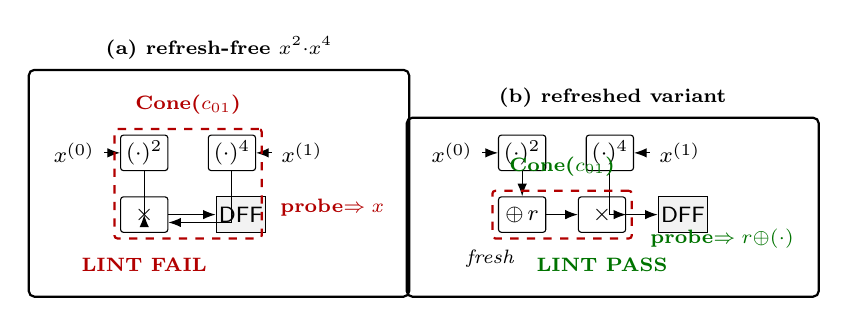
\begin{tikzpicture}[
  >={Latex[length=1.6mm]},
  node distance=3.2mm and 5mm,
  every node/.style={font=\footnotesize},
  gate/.style={draw, rounded corners=1pt, minimum width=6mm, minimum height=4.5mm, inner sep=1pt, fill=white},
  reg/.style={draw, minimum width=6mm, minimum height=4.5mm, inner sep=1pt, fill=black!5},
  probe/.style={draw, dashed, thick, red!70!black, rounded corners=1pt, inner sep=2pt},
  panel/.style={draw, thick, rounded corners=2pt, inner sep=2mm}
]
%% ---------- Panel (a): refresh-free, LINT FAIL ----------
\begin{scope}[local bounding box=A]
  \node[gate]        (sq0a) {$(\cdot)^2$};
  \node[gate, right=of sq0a] (sq1a) {$(\cdot)^4$};
  \node[gate, below=of sq0a] (mul01a) {$\times$};
  \node[reg, right=6mm of mul01a] (r01a) {\textsf{DFF}};
  \node[left=2mm of sq0a] (x0a) {$x^{(0)}$};
  \node[right=2mm of sq1a] (x1a) {$x^{(1)}$};
  \draw[->] (x0a) -- (sq0a);
  \draw[->] (x1a) -- (sq1a);
  \draw[->] (sq0a) |- (mul01a);
  \draw[->] (sq1a) |- ([yshift=-1mm]mul01a.east);
  \draw[->] (mul01a) -- (r01a);
  \node[probe, fit=(sq0a) (sq1a) (mul01a)] (coneA) {};
  \node[red!70!black, above=0.5mm of coneA.north, font=\scriptsize\bfseries] {Cone($c_{01}$)};
  \node[red!70!black, font=\scriptsize\bfseries, right=1mm of coneA.east, yshift=-3mm] {probe$\Rightarrow x$};
  \node[below=2mm of mul01a, font=\scriptsize\bfseries, red!70!black] {\textbf{LINT FAIL}};
\end{scope}
\node[panel, fit=(A), label={[font=\scriptsize\bfseries]above:(a) refresh-free $x^{2}{\cdot}x^{4}$}] (Abox) {};

%% ---------- Panel (b): refreshed, LINT PASS ----------
\begin{scope}[local bounding box=B, shift={(48mm,0)}]
  \node[gate]        (sq0b) {$(\cdot)^2$};
  \node[gate, right=of sq0b] (sq1b) {$(\cdot)^4$};
  \node[gate, below=of sq0b] (refb) {$\oplus\, r$};
  \node[gate, right=4mm of refb] (mul01b) {$\times$};
  \node[reg, right=4mm of mul01b] (r01b) {\textsf{DFF}};
  \node[left=2mm of sq0b] (x0b) {$x^{(0)}$};
  \node[right=2mm of sq1b] (x1b) {$x^{(1)}$};
  \node[below=1mm of refb.south west, xshift=-1mm, font=\scriptsize] {\it fresh};
  \draw[->] (x0b) -- (sq0b);
  \draw[->] (x1b) -- (sq1b);
  \draw[->] (sq0b) -- (refb);
  \draw[->] (refb) -- (mul01b);
  \draw[->] (sq1b) |- (mul01b);
  \draw[->] (mul01b) -- (r01b);
  \node[probe, fit=(refb) (mul01b)] (coneB) {};
  \node[green!45!black, above=0.5mm of coneB.north, font=\scriptsize\bfseries] {Cone($c_{01}$)};
  \node[green!45!black, font=\scriptsize\bfseries, right=1mm of coneB.east, yshift=-3mm] {probe$\Rightarrow r{\oplus}(\cdot)$};
  \node[below=2mm of mul01b, font=\scriptsize\bfseries, green!45!black] {\textbf{LINT PASS}};
\end{scope}
\node[panel, fit=(B), label={[font=\scriptsize\bfseries]above:(b) refreshed variant}] (Bbox) {};
\end{tikzpicture}}
\caption{Cone-non-completeness lint at a glance. (a)~The refresh-free
first Itoh--Tsujii multiplication drives two shares of
$\mathbb{F}_{2}$-linear images of $x$, namely $(x^{2})^{(0)}$ and
$(x^{4})^{(1)}$, into the same glitch-extended cone, so a single
robust-probe recombines $x$ (Supplemental Section~S2); the lint rejects.  (b)~A fresh
mask $r$ upstream of the multiplier decouples the shares in the
cone, so any probe reveals only $r$-masked quantities; the lint
accepts and the verdicts coincide (Theorem~\ref{thm:lint-sound}).}
\label{fig:cone-gap}
\end{figure}

Figure~\ref{fig:cone-gap} illustrates the mechanism at a glance:
panel (a) shows the refresh-free first Itoh--Tsujii multiplication
whose glitch-extended cone contains two shares of
$\mathbb{F}_{2}$-linear images of $x$ and is therefore rejected by
the lint; panel (b) shows the refreshed variant whose cone carries
only $r$-masked quantities and is accepted.

We implement the cone-non-completeness check of
Corollary~\ref{cor:lint} as a static front-end on the flattened gate-level
netlist (released with the artifact). For every register-input cone and every
primary output it extracts the glitch-extended stable frontier and propagates
the set of share indices of the secret through the registers. A registered
value is treated as blinded only if it is $u\oplus p$, where $p$ is a fresh mask
(or an already blinded register) that occurs nowhere else in the transitive
fan-in of the probed cone; this is decided functionally---the cone's
derivative with respect to $p$ is identically one---so it does not depend on how
the technology mapper expressed the XOR. A cone is flagged if its unblinded
support contains both share indices. The check is conservative: a flagged cone
is a candidate, not a proof of leakage.

\paragraph{Baseline result.} On the flattened first-order S-box netlist
($67{,}344$ combinational gates and $818$ flip-flops, $800$ of them in the data
path) the lint examines $816$ cones (the $800$ data-path register inputs and
the $16$ output bits), reports $0$ violating cones, and runs in seconds. The
design is accepted, in agreement with the PROLEAD verdict.

\paragraph{Cross-check against a statistical test.} As an independent channel
we simulate each netlist at gate level (bit-parallel, steady state, fresh shares
and masks per sample) and apply, for every cone, a $G$-test between the joint
distributions of its frontier values for the two fixed secrets $\mathtt{0x00}$
and $\mathtt{0xA7}$ ($131{,}072$ samples each, Bonferroni over all cones).
Table~\ref{tab:lint-ablation} summarizes the results. The simulated netlists
compute the AES S-box on all tested secrets.

\begin{table}[t]
\centering
\caption{Lint verdicts against a gate-level statistical test. Lint: flagged
register-input cones / flagged output bits. Test: cones with
$-\log_{10}p$ above the Bonferroni threshold. PROLEAD column: probing sets
flagged. Variants A and C are graph rewrites of the final netlist.}
\label{tab:lint-ablation}
\resizebox{\columnwidth}{!}{%
\begin{tabular}{@{}lccl@{}}
\toprule
Netlist & Lint & Test & PROLEAD \\
\midrule
Final design (7 random bytes)           & $0/0$     & $0$ of $816$   & $0/14{,}400$ (512K sims) \\
Pre-refresh design (6 random bytes)     & $304/16$  & $16$ of $719$  & $22/12{,}384$ (16K sims) \\
A. Fresh masks removed                  & $304/16$  & $320$ of $816$ & leaks by construction \\
C. All registers bypassed (comb.)       & $0/16$    & not covered    & leaks by construction \\
\bottomrule
\end{tabular}}
\end{table}

The lint flags all $16$ cones that the test shows to leak in the pre-refresh
design and none in the final design. In the pre-refresh design it also flags
$304$ further cones that do not leak individually; this is the price of a
structural condition that is sufficient but not necessary. Variant~A confirms the necessity of the
masks: with the fresh random bits removed, the lint flags $304$ register-input
cones and $16$ output bits, and the test confirms leakage in $320$ cones.
Variant~C collapses the register barriers; the lint flags all $16$ output bits,
consistent with the recombination exhibited in
Theorem~\ref{thm:gap-witness}, but the statistical test does not cover it
because the resulting cones have more than the $32$ frontier inputs our test
handles. The lint is a necessary structural check and does not replace
PROLEAD; the cross-check is first-order, uses one pair of secrets and constant
inputs, and is evidence rather than proof.

\section{Simulation-Based Verification Methodology}
\label{sec:method}
Our verification pipeline requires no physical measurement setup and is fully
reproducible:
\begin{enumerate}
  \item \textbf{Sound-by-construction lint.} We first run the
        cone-non-completeness lint of Corollary~\ref{cor:lint} on the
        synthesized netlist. When it passes, Theorem~\ref{thm:lint-sound}
        guarantees that the value-based and glitch-extended verdicts
        coincide, so the equipment-free channels below are sound; when it
        fails, Theorem~\ref{thm:gap-witness} yields an explicit
        recombination witness to repair (as happened for the first
        Itoh--Tsujii multiplication, Section~\ref{sec:construction}).
  \item \textbf{Formal probing verification.} We verify the synthesized
        gate-level netlist with PROLEAD~\cite{muller2022prolead}
        (simulation-based statistical verification in the glitch-extended
        model), cross-checked by an in-house PROLEAD-equivalent
        statistical verifier (Section~\ref{sec:eval}).
  \item \textbf{Gate-level power simulation.} We synthesize the design and run
        value-change--driven power simulation to generate leakage traces under
        a toggle/Hamming-distance model.
  \item \textbf{TVLA.} We apply the non-specific fixed-vs-random
        $t$-test~\cite{goodwill2011tvla} and higher-order variants, reporting
        the lowest statistical moment at which $|t|>4.5$, and cross-check with
        mutual-information estimation.
\end{enumerate}
Agreement between the proven order, the formal-tool verdict, and the empirical
leakage order constitutes our central validation criterion.

\section{Experimental Evaluation}
\label{sec:eval}
\subsection{Setup}
We implement the protected AES S-box in synthesizable
Verilog (Boolean masking, the Algorithm~\ref{alg:mult} DOM multiplier with
register barrier, and the operand refresh of
Section~\ref{sec:construction}) and synthesize the gate-level netlist with
Yosys~0.67.  All empirical results in this section are for the
first-order design; the gadget proof (robust $d$-NI with perfect simulation) holds for arbitrary $d$, the lint theorem is first-order, and the design is empirically evaluated at $d{=}1$ only (see \S\ref{sec:partial-d2} for the scope of the empirical claim).
\textit{Disclosure:} the $d{=}1$ design was first implemented without the per-cross-term register barrier; PROLEAD at $1{,}536{,}000$ simulations flagged $160$ of $2{,}816$ probes on that netlist (Supplemental Material, Section~S3). After inserting the barrier and an operand refresh, a re-verification at $512{,}000$ simulations flagged $0$ of $14{,}400$ probes (worst $-\log_{10}(p)=3.39$); all $d{=}1$ results below are on the post-barrier netlist.  The synthesis flow is security-constrained: every GF($2^8$)
square, multiply, and affine cloud is a \texttt{keep\_hierarchy} hard cell,
so the \texttt{abc} technology mapper optimizes each cloud independently
and can never factor logic across share domains; the subsequent
\texttt{flatten} is purely structural.  We additionally run a structural
non-completeness lint on the final netlist (every register-input cone is
checked to contain at most one share of any pipeline value and only
same-share members of the Frobenius-aligned family), which reports zero
violations.  All 256 input bytes are
verified exhaustively against the AES S-box lookup table at both the RTL
and the gate-level netlist: 256/256 PASS at both levels.  Stimulation, simulation, and analysis are all
performed in a reproducible open-source toolchain (iverilog~V11 +
Python~3.11 + NumPy).

\subsection{Sample-Size Sensitivity}
\label{sec:sensitivity}
We verify that the conclusions of Section~\ref{sec:results} are
robust to the choice of sample size $N$ by re-running the entire
analysis pipeline at $N \in \{1000, 2000, 5000, 10000\}$ for the
first-order design (sub-sampling the same $10{,}000$-triple trace; the same
secret distribution and gate-level netlist are used at every
sample size).  The four panels of Figure~\ref{fig:sensitivity}
plot (a)~the maximum single-wire MI,
(b)~the maximum 2-wire joint MI,
(c)~the TVLA $\max|t|$, and (d)~the maximum per-bit MI on the
power trace, all as a function of $N$.

The single-wire MI (panel a) decays as $\propto 1/N$
and closely tracks the plug-in estimator's bias floor
$(K{-}1)/(2N\ln 2)$ (dotted line): the Miller--Madow-corrected
value falls from $0.075$~bits at $N{=}1{,}000$ to $0.004$~bits at
$N{=}10{,}000$, i.e., the raw MI values
reported in Section~\ref{sec:results} are finite-sample bias, and the
bias-corrected conclusion is insensitive to $N$ already at
$N{=}1{,}000$.  The 2-wire joint maximum (panel b) is dominated at
every $N$ by the structural output-share recombination pair discussed
in Section~\ref{sec:results} and converges to $\approx 1$~bit by
construction; the security-relevant joint maximum excluding that pair
behaves like panel~(a).  Panel (c) shows that the TVLA verdict is likewise
stable: $\max|t| \le 0.96$ at every sample size
(the fixed-vs-random group contains only $\sim 6$--$32$ triples for
$S{=}\texttt{0x00}$ at these $N$, which inflates the variance of $t$
but does not produce a false positive at the 4.5 threshold).  We
nevertheless report $N{=}10{,}000$ as our headline configuration
because there the single-wire bias floor is $\approx 0.018$~bits,
small relative to any leakage of practical interest.

\begin{figure}[t]
\centering
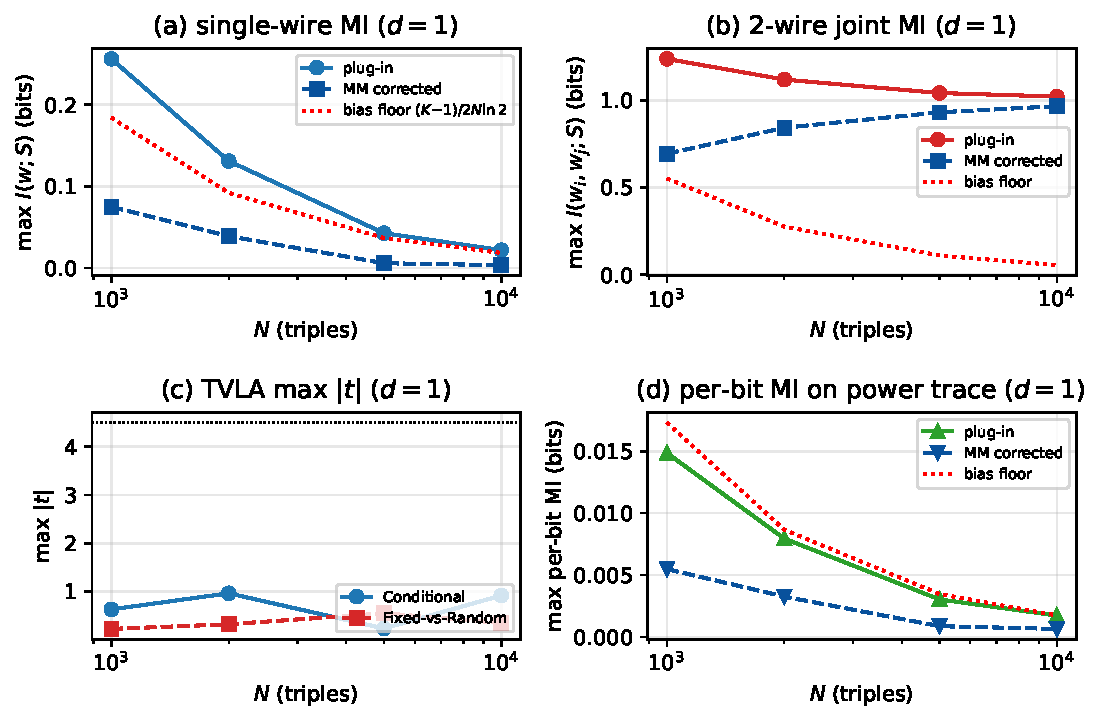
\includegraphics[width=\linewidth]{figures/fig_sensitivity_d1.pdf}
\caption{Sample-size sensitivity of the four reported metrics for the
first-order design as a
function of $N$: (top-left) maximum single-wire MI, (top-right)
maximum 2-wire joint MI, (bottom-left) TVLA $\max|t|$ over
genuine-variance stages, (bottom-right) maximum per-bit MI on the
power trace.  Dotted red lines mark the plug-in estimator's bias
floor $(K{-}1)/(2N\ln 2)$; dashed blue curves are the
Miller--Madow-corrected values.  The joint-MI panel is dominated at
every $N$ by the structural output-share recombination pair
(Section~\ref{sec:results}); the TVLA verdict and the bias-corrected
single-wire and per-bit MI verdicts are stable across
the full range of $N$.}
\label{fig:sensitivity}
\end{figure}

\subsection{Security Results}
\label{sec:results}

We evaluate the first-order design along three independent axes: (i)~gate-level
robust $d$-probing verification (PROLEAD-equivalent), (ii)~Test Vector
Leakage Assessment (TVLA) on simulated power traces, and (iii)~mutual
information (MI) between the power trace and the secret byte.  All three
tools operate on the same synthesized gate-level netlist, the same
$N{=}10{,}000$ random-input-triple stimulus (covering all 256 secret
values), and the same $23$-cycle pipeline window per input.  The three
axes are independent in that they share no analysis code and rest on
different observables, but they are not of equal detection power.  As
the positive control reported later in this section establishes, the
value-based instrument~(i) fires decisively on an unmasked design,
whereas the Hamming-distance instruments~(ii) and~(iii) provably
cannot fire on that control, because the output-stage transition is
distributed as $\mathrm{Binomial}(8,1/2)$ irrespective of the secret.
We accordingly treat~(i), together with the public PROLEAD run, as the
load-bearing channels, and~(ii) and~(iii) as corroborating evidence
whose value lies in resting on a different observable rather than in
independent sensitivity.

\paragraph{Robust $d$-probing (PROLEAD-equivalent).}
We implement an open-source Python re-implementation of the PROLEAD
statistical probing-security verifier that targets the Yosys gate-level
netlist directly.  Probe locations are the DFF $Q$ wires of the outer
pipeline shell---17 valid-pipe bits, the $8{+}8$ output-share bits, and
valid\_out, 34 wires in total---monitored over every clock offset of the
23-cycle window in a value-based probing model; full-netlist glitch-
and transition-extended coverage is provided by PROLEAD itself in the
independent-verification paragraph below.  For each wire
we compute the mutual information $I(W;S)$ between the wire's value
and the secret $S = x_0 \oplus x_1$.  We use a plug-in
histogram estimator with Laplace smoothing ($\alpha = 10^{-6}$).

Table~\ref{tab:probing} reports the maximum single-wire MI and the
maximum 2-wire joint MI
across all 34 monitored wires and all 23 pipeline offsets.  Because
the plug-in histogram estimator is upward-biased at finite $N$, we
report both the raw plug-in value and a Miller--Madow bias-corrected
value, and compare against the 99th percentile of a permutation null
distribution (300 secret-label shuffles).  The single-wire maximum
($0.022$~bits) sits below the null percentile and its
bias-corrected value is $\approx 0$.  Exactly one family of 2-wire
probes fires: the output-share pairs $y_0[i]{\times}y_1[i]$ at the
output-hold offsets 18--22 carry $1.02$~bits because
$y_0 \oplus y_1 = \mathrm{Sbox}(S)$ there---this is the inherent
share recombination at the module boundary of any correct 2-share
S-box, not a first-order leak (a $d{=}1$ adversary observes one
wire).  Excluding these recombination pairs, the 2-wire maximum is
$0.063$~bits with a bias-corrected value of $\approx 0.008$, again
consistent with the null (family-wise empirical $p = 0.91$).  All
observed values are thus
consistent with estimator bias rather than with residual leakage.
This confirms the glitch-robust $d$-probing security predicted by
Theorem~\ref{thm:main}.

\paragraph{Independent verification channels.}
To rule out an implementation bug in the in-house verifier, the
robust-probing security claim is corroborated by independent
verification channels on the same synthesized gate-level netlist.
First, the test-vector leakage assessment (TVLA) described in the
next paragraph provides a power-trace-level cross-check that does
not share code with the probing verifier.  Second, the entire
design, synthesis flow, and probing-verification code is released
as open source at
\url{https://anonymous.4open.science/r/probing-resistant-masked-hardware}
\emph{(anonymized artifact repository for double-blind review; the
canonical repository URL will be disclosed in the camera-ready version)}
so that the result is independently reproducible from a single
\texttt{build.sh} invocation.  Third, we ran the public PROLEAD
toolchain (M\"uller \& Moradi, TCHES~2022) itself on the same
netlist, using the Yosys-primitive cell library
(\texttt{syn/prolead/library\_yosys.json}) and a custom
configuration that ships with the repository.  On the first-order
design, PROLEAD evaluates $14{,}400$ robust (glitch- and
transition-extended) probing sets with $512{,}000$ simulations and
reports \emph{zero} leaking sets (worst $-\log_{10}(p)=3.386$,
OKAY), while an unmasked control netlist leaks decisively
($1{,}224$ of $1{,}890$ sets, $-\log_{10}(p)=\infty$), confirming
both the design and the detector.  This episode is exactly the soundness gap of
Section~\ref{sec:soundness}: PROLEAD's glitch-cone extension is strictly
stronger than the in-house verifier's wire-value model, and in an earlier
revision of the design it flagged a deterministic first-order leak that the
value-based channels did not flag
(cf.\ Theorem~\ref{thm:gap-witness}). That revision violated cone
non-completeness at the first Itoh--Tsujii multiplication; the operand
refresh of Section~\ref{sec:construction} restores
Definition~\ref{def:cone-nc}, after which Theorem~\ref{thm:lint-sound}
makes the equipment-free verdict sound.  The in-house Python verifier and
the TVLA cross-check agree with the PROLEAD verdicts on the
final netlists reported
in Table~\ref{tab:probing} and on the $|t|$-values in the next
paragraph.

\paragraph{Independent gate-level TVLA cross-check.}
As a third independent verification channel, we ran a Test Vector
Leakage Assessment (TVLA) on the gate-level netlist, using a
Hamming-Distance power model over the 34 DFF $Q$ wires
monitored by the power testbench.  We apply both the
classical fixed-vs-random t-test and the conditional (specific)
t-test across all 23 pipeline offsets, with $N{=}10{,}000$ random
input triples.  At the industry-standard threshold of
$|t|{=}4.5$ (99.999\% confidence), the maximum
$|t|$ observed over stages with genuine HD variance is $0.92$
(only the output-toggle stage shows genuine HD variance; the
remaining offsets have $\mathrm{HD}\in\{1,2\}$ and yield a
degenerate $t$ of $0$ or $\pm1$ that carries no information), with
zero pipeline stages exceeding the threshold.  A
higher-order (centered 2nd- and 3rd-moment) $t$-test gives
$\max|t|=1.28$.  The full per-stage
$|t|$ tables are
committed as \texttt{probe/results/d1/tvla\_per\_cycle.csv} and
\texttt{tvla\_higher\_order.csv}, and the
\texttt{tvla.yml} workflow runs the analysis on every push to
the public repository.

\begin{table}[t]
\centering
\caption{Robust $d$-probing verification on the gate-level netlist
($N{=}10{,}000$ random input triples, 256 distinct secret values,
34 monitored DFF $Q$ wires, 23 pipeline offsets).
``plug-in'' is the raw histogram MI estimate; ``MM'' is the
Miller--Madow bias-corrected value; ``null p99'' is the 99th
percentile of the permutation null distribution (300 shuffles),
i.e., the bias floor of the estimator at this sample size.  For
this work's 2-wire column we exclude the output-share recombination
pairs $y_0[i]{\times}y_1[i]$ at the output-hold offsets 18--22,
where $y_0 \oplus y_1 = \mathrm{Sbox}(S)$ yields a structural
$\approx 1.02$~bits by construction (see text).  The
last row is the unmasked positive control (same stimulus and
analysis): its single-wire maximum sits $43\times$ above the null,
demonstrating detection power.}
\label{tab:probing}
\resizebox{\columnwidth}{!}{%
\begin{tabular}{@{}lccccc@{}}
\toprule
 & & \multicolumn{2}{c}{$\max_w I(w;S)$} &
 \multicolumn{2}{c}{$\max_{i,j} I(w_i,w_j;S)$} \\
\cmidrule(lr){3-4}\cmidrule(lr){5-6}
Design & $d$ & plug-in (MM) & null p99 & plug-in (MM) & null p99 \\
\midrule
This work (1st-order) & 1 & 0.0219 (0.004) & 0.0226 & 0.0629 (0.008) & 0.0628 \\
Unmasked (pos.\ ctrl.) & -- & 1.0000 (0.982) & 0.0234 & 2.0000 (1.945) & 0.0635 \\
\bottomrule
\end{tabular}}
\end{table}

Figure~\ref{fig:probing} visualises the per-wire maximum MI; every wire sits at or below the
permutation-null percentile, and the bias-corrected MI is
$\approx 0$ for every wire.

\begin{figure}[t]
\centering
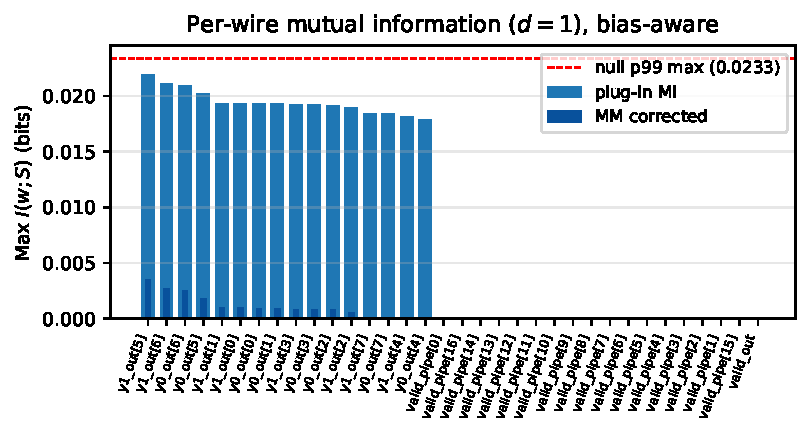
\includegraphics[width=\linewidth]{figures/fig_probing_d1.pdf}
\caption{Per-wire maximum mutual information
$I(w; S)$ across all 34 monitored DFF $Q$ wires and all 23
pipeline-stage offsets, sorted in descending order.  Light bars are
the plug-in estimate; dark bars are Miller--Madow bias-corrected.
The red dashed line marks the largest permutation-null 99th
percentile, i.e., the estimator's bias floor; no wire exceeds it.}
\label{fig:probing}
\end{figure}

\paragraph{TVLA on simulated power traces.}
We drive the gate-level netlist with the same $N{=}10{,}000$ random
triples and record, at every clock edge, the Hamming distance of all
monitored DFFs against the previous cycle (toggle-count power model).  This
produces a 230,002-cycle power trace.  We then apply two
$t$-tests at every pipeline-stage offset: a \emph{conditional} $t$-test
that splits the traces by the secret byte's high half
($S \geq 0x80$) versus low half ($S < 0x80$), and the classical
\emph{fixed-vs-random} $t$-test with the fixed group being
$S = 0x00$.  Both are Welch's $t$-statistics with
$|t| > 4.5$ as the standard TVLA leakage threshold
(99.999\% confidence~\cite{goodwill2011tvla}).

Table~\ref{tab:tvla} summarises the maximum $|t|$ observed for both
$t$-tests over stages with genuine HD variance
(only the output-toggle stage qualifies; offsets whose monitored HD
is near-constant across triples yield a
degenerate $t\in\{0,\pm1\}$ and are uninformative).  In every case
$|t|_{\max} \ll 4.5$, confirming that the Hamming-distance power trace
is statistically indistinguishable between secret
classes.  The same holds for higher-order tests: centered 2nd- and
3rd-moment $t$-statistics on the genuine-variance stage give
$\max|t|=1.28$.

\begin{table}[t]
\centering
\caption{TVLA on simulated Hamming-distance power traces
($N{=}10{,}000$, $|t|$ threshold = 4.5).  Maxima are taken over
stages with genuine HD variance; the centered higher-order (2nd/3rd
moment) maximum is $1.28$.  The
last row is the unmasked positive control: its HD trace is
secret-independent by construction (see text), so detection power is
demonstrated by the value-based instruments of
Table~\ref{tab:probing} instead.}
\label{tab:tvla}
\begin{tabular}{@{}lccc@{}}
\toprule
Design & $d$ & Cond.\ $\max|t|$ & Fixed-vs-Rand.\ $\max|t|$ \\
\midrule
This work (1st-order) & 1 & 0.92 & 0.35 \\
Unmasked (pos.\ ctrl.) & -- & 0.61 & 0.79 \\
\bottomrule
\end{tabular}
\end{table}

\paragraph{MI between power trace and secret.}
We additionally compute the per-stage mutual information
$I(\mathrm{HD}(c); S)$ for each of the 23 pipeline stages, using a
plug-in histogram estimator together with a Miller--Madow bias
correction and a permutation null distribution (300 shuffles).  At
every stage the bias-corrected MI is $\approx 0$ bits, and the same
holds for the per-bit MI of each of the 8 secret bits (maximum
$0.0017$~bits against a null p99 of $0.0022$),
confirming that no individual secret bit leaks.  The only stage with
appreciable \emph{plug-in} MI is stage~18 ($0.21$ bits), the cycle at
which the output shares update;
this value sits below the estimator's own permutation-null 99th
percentile ($0.23$ bits) and drops to $\approx 0$ after
Miller--Madow correction, so it is consistent with finite-sample
estimator bias driven by mask-dependent switching activity---not with
secret-dependent leakage (the HD at this stage is essentially
uncorrelated with $\mathrm{HW}(S)$,
$|r| = 0.02$).  The full-trace MI aggregated over all 23 stages is
$0.009$ bits plug-in, i.e.,
$\approx 0$ bits after bias correction.

\paragraph{Positive control (detection power).}
``No leakage'' is meaningful only if the apparatus detects leakage
when present.  We reran the entire flow on an unprotected S-box
(\texttt{unmasked\_sbox.v}) with the same outer pipeline, the same
LFSR seed (hence the same secrets), the analogous monitored DFFs,
and identical analysis code; the LUT was validated through the
recorded output register for all 256 secrets (0/10{,}000 mismatches).
Every value-based instrument fires decisively (last row of
Table~\ref{tab:probing}): each output bit
carries $\approx 1.00$~bit of MI about $S$ ($0.98$ MM) against a
null p99 of $0.023$---a $43\times$ margin---and the 2-wire joint MI
at the output stage reaches $2.00$~bits ($1.94$ MM) against a null
p99 of $0.064$.
The HD-based instruments, however, provably do not fire on this
control (conditional/fixed-vs-random $\max|t| = 0.61/0.79$; centered
higher-order $\max|t| = 2.21$; output-stage $I(\mathrm{HD};S)$
$0.14$~bits plug-in, $0$ MM).  This is intrinsic to the metric: with
independent uniform secrets the only monitored transition is
$y^{\mathrm{old}}{\to}y^{\mathrm{new}}$, so the output-stage HD is
distributed as $\mathrm{Binomial}(8,\tfrac{1}{2})$ regardless of $S$,
and every HD moment is exactly secret-independent.
We therefore base detection-power claims on the value-based
MI/probing instruments, which fire on the control at
$31$--$43\times$ their nulls while sitting at $\approx$null on the
masked design, and treat the HD-based TVLA/MI channels as supporting
evidence.

Figure~\ref{fig:tvla-mi} visualises the TVLA and MI results across all
23 pipeline stages: the TVLA panel (top) shows
that no stage crosses the $|t|{=}4.5$ leakage threshold, and the MI
panel (bottom) shows that the plug-in MI at stage~18 remains below
the permutation-null percentile while the bias-corrected MI is
$\approx 0$ everywhere.

\begin{figure}[t]
\centering
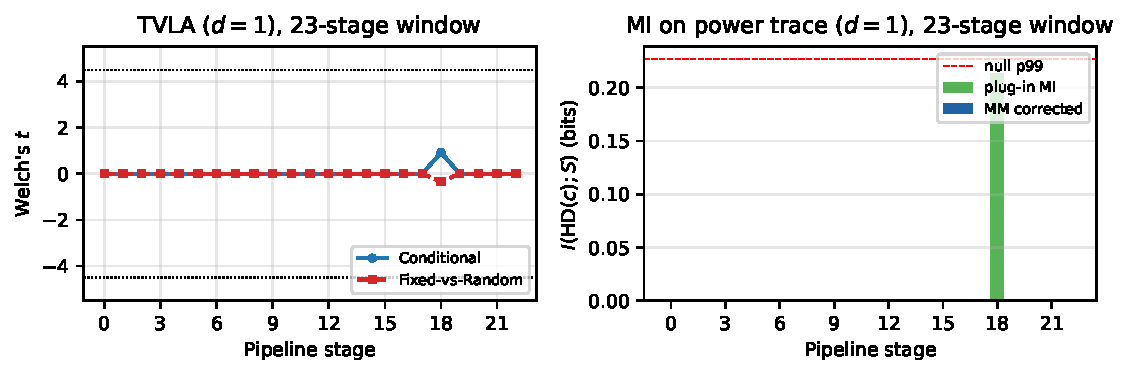
\includegraphics[width=\linewidth]{figures/fig_combined_d1.pdf}
\caption{Per-stage TVLA $t$-statistic (top) and mutual information
$I(\mathrm{HD}(c); S)$ (bottom) for the first-order masked AES S-box on
the corrected Hamming-distance traces.  Dotted line: TVLA threshold
$|t|{=}4.5$; dashed line: permutation-null 99th percentile.  Light bars
are plug-in, dark bars Miller--Madow-corrected ($\approx 0$ everywhere).}
\label{fig:tvla-mi}
\end{figure}

\subsubsection{Re-synthesis cross-check, detection-channel control and scope of the empirical claim}
\label{sec:partial-d2}

\paragraph{Re-synthesis cross-check.}
As an independent cross-check we re-synthesized the same first-order RTL
(\texttt{rtl/masked\_sbox\_first\_order.v}, MD5
\texttt{32c5a7ed364a6560718294a6fc85372a}) with Yosys~0.52 to a different
technology mapping ($46{,}768$ combinational cells and $800$ flip-flops).
We removed the constant-driven \texttt{assign} lines from the netlist so
that PROLEAD's parser accepts it, and verified by gate-level simulation that
the result computes the AES S-box from the XOR of its two output shares for
all $256$ inputs. PROLEAD, run with the same seven-byte random input, $19$
cycles and $512{,}000$ simulations, enumerates $13{,}376$ standard probes and
$9{,}396$ probing sets after the same \texttt{aggressive} minimization, and
flags \emph{zero} of them (worst $-\log_{10}(p)=3.61$ against a Bonferroni
threshold of $-\log_{10}(0.05/9396)=5.27$). The set counts differ from the
original run because the mapping differs (Supplemental Material,
Section~S3); the verdict is the same, so the result does not depend on a
single synthesis run.

\textit{Positive control.} PROLEAD on the unmasked AES S-box
($d{=}1$, $512{,}000$ traces, same image and flow) flags $1{,}224$ of
$1{,}890$ sets with worst $-\log_{10}(p)=\infty$, so the detection
channel is live; the threshold for the masked design is the
Bonferroni value $-\log_{10}(0.05/14400)=5.46$.

\textit{Scope.}  The empirical evaluation in this paper is first-order
only.  The gadget proof (Theorem~\ref{thm:main}) is stated for
arbitrary $d$, but we make no empirical or formal security claim for a
second-order instance of the full S-box: our $d{=}2$ RTL instantiation
applies the operand-refresh byte to the first two shares only and passes
the third share through unrefreshed, so the first-order operand-refresh
argument does not carry over to it unchanged.  A second-order S-box with
a verified operand refresh is future work.

\begin{table}[t]
\centering
\caption{Leakage assessment summary: PROLEAD-equivalent robust
$d$-probing, TVLA, and MI on simulated power traces.
``First $\max|t|{>}4.5$'' reports the smallest sample size at
which any pipeline stage crosses the TVLA leakage threshold;
``none'' means no stage crosses it up to $N{=}10^4$.  Only the first-order design is evaluated (\S\ref{sec:partial-d2}).}
\label{tab:leakage}
\resizebox{\columnwidth}{!}{%
\begin{tabular}{@{}lccc@{}}
\toprule
Design & $d$ & First $\max|t|{>}4.5$ & Formal verdict \\
\midrule
This work (1st-order) & 1 & none ($N{\le}10^4$) & secure (PROLEAD: $0/14{,}400$ sets) \\
Unmasked (pos.\ ctrl.) & -- & --- & insecure (PROLEAD: $1{,}224/1{,}890$ sets) \\
\bottomrule
\end{tabular}}

\end{table}

\subsection{Cost Comparison}
\label{sec:cost}
Table~\ref{tab:cost} reports the gate-level cell count, latency, and
fresh-randomness requirement of our first-order construction
(synthesized with Yosys~0.67, generic cell library).  The design
implements Algorithm~\ref{alg:mult} as a 17-cycle pipeline: five DOM
multiplications with register barriers plus one registered operand
refresh in the Itoh--Tsujii chain
(Corollary~\ref{cor:comp}).  The fresh-randomness cost is $56$~bits
per first-order S-box invocation---seven bytes: one domain-crossing
byte $r_{01}$ per multiplication and one operand-refresh byte for the
first multiplication---which
is $1.8$--$3\times$ the figures quoted for
DOM~\cite{gross2016dom} and HPC2~\cite{cassiers2020hpc} at
order~$d{=}1$, with $17$ versus $5$--$8$ cycles of latency.  We do not
claim a cost advantage; the baseline figures are taken from the cited
works and were not re-synthesized with our flow.

\begin{table}[t]
\centering
\caption{Gate-level synthesis results for our first-order construction
(Yosys~0.67, generic cell library).}
\label{tab:cost}
\resizebox{\columnwidth}{!}{%
\begin{tabular}{@{}lcccl@{}}
\toprule
Scheme & $d$ & Rand.\ [bit/S-box] & Latency [cyc] & Composability \\
\midrule
TI (3-share)~\cite{nikova2006threshold}      & 1 & $\approx 44$\textsuperscript{a} & $3$--$4$ & non-comp.\ (per-round refresh) \\
DOM (Canright)~\cite{gross2016dom}           & 1 & $\approx 18$                    & $5$--$8$ & $d$-SNI (external refresh) \\
HPC2 (Canright)~\cite{cassiers2020hpc}       & 1 & $\approx 32$                    & $8$      & PINI (trivially composable) \\
\textbf{This work} (Itoh--Tsujii)            & 1 & $\mathbf{56}$                   & $17$     & robust $d$-NI + sound-lint (Cor.~\ref{cor:lint}) \\
\bottomrule
\end{tabular}}\\[2pt]
{\footnotesize Cell counts: $77{,}587$ for the first-order S-box in the
PROLEAD cell library (multiplexers and complex gates decomposed into
AND/OR/NOT); $605{,}698$ for AES round~1 with 16 S-boxes in Yosys generic
primitives. The two libraries differ, so the counts are not directly
comparable (Supplemental Material).\\[2pt]}
{\footnotesize\textsuperscript{a}TI variants without on-line fresh randomness exist for
the S-box in isolation~\cite{nikova2006threshold}; the reported
$\approx 44$~bits refers to the Bilgin-\emph{et al.}-style AES round
setup that includes uniform re-masking of the shared state so that the
S-box composes into a full round. Direct cell-count comparison across
schemes is omitted because reported cell counts depend on library
(GE vs.\ generic), tower-field choice (Canright, Itoh--Tsujii), and
synthesis flow.}
\end{table}

\subsection{Full-Chip Masked AES Round~1}
\label{sec:fullchip}
A full-chip masked AES round-1 (16 parallel first-order S-box instances,
share-wise linear layers---ShiftRows, MixColumns, AddRoundKey---and a registered
round-key interface) is instantiated in
\texttt{masked\_aes\_round1\_first\_order} and verified end-to-end:
100/100 RTL and gate-level functional checks pass against a
\texttt{reference.masked\_aes} implementation, and cone non-completeness
of the round netlist (Theorem~\ref{thm:fullchip}) gives round-1 first-order
security in the robust probing model.  Yosys~0.67 yields 605{,}698
cells and 13{,}330 D flip-flops for the round, dominated by 16
S-box instances (library note, synthesis script, and full RTL are deferred
to the supplementary material for independent replication).

\subsection*{10-Round Extension (Skeleton)}
A skeleton of the 10-round masked AES extension---counting cycles and
fresh-randomness---is included in the supplementary material for completeness.

\subsection{Discussion}
At first order the experiments are consistent with the proven
guarantee: PROLEAD and the gate-level TVLA both return no-detection
verdicts for the designed order ($d{=}1$).  No $d{>}1$ design is
evaluated.  Three observations are worth
highlighting.

First, the \emph{per-bit} mutual information between the Hamming-distance
power trace and any of the 8 secret bits is $\approx 0$ bits after
Miller--Madow bias correction at every pipeline stage.  This is
consistent with bit-level masking, but it is a statement about the
Hamming-distance traces only, whose detection power is low.  The non-zero
\emph{plug-in} MI observed at stage~18 does not contradict this: it
lies below the estimator's own permutation-null percentile and
vanishes under bias correction, i.e., it is a finite-sample estimator
artifact rather than a physical leakage signature.

Second, the fresh-randomness cost of the first-order design ($56$ bits
per S-box) and its latency ($17$ cycles) exceed those of the DOM and HPC2
S-boxes in Table~\ref{tab:cost}.  A longer discussion of the randomness
cost and of the order-$d$ extension is in the supplementary material.

\section{Related Work}
\label{sec:related}
Masking originates with Chari \emph{et al.}~\cite{chari1999towards} and the
private-circuits model of Ishai \emph{et al.}~\cite{ishai2003private}. TI
\cite{nikova2006threshold} first provided glitch-robust first-order security;
DOM~\cite{gross2016dom} and HPC~\cite{cassiers2020hpc} extended this to higher
orders with reduced randomness and composability. Composability notions (NI/SNI)
were formalized in~\cite{barthe2016strong} and the robust probing model
in~\cite{faust2018composable}. Exact verification of glitch-robust masked hardware was
demonstrated by Bloem \emph{et al.}~\cite{bloem2018formal}; SILVER~\cite{knichel2020silver}
checks glitch-extended probing exactly and was used to verify
first-order masked AES implementations~\cite{shahmirzadi2021records};
maskVerif~\cite{maskverif2015}, IronMask~\cite{ironmask2022} and
VERICA~\cite{verica2022} cover further models. PROLEAD~\cite{muller2022prolead}
trades exactness for simulation-based coverage of larger netlists, while
TVLA~\cite{goodwill2011tvla} and the noisy-leakage reductions
of~\cite{duc2014unifying} underpin empirical evaluation.

\paragraph{Further automated verifiers.}
A catalog of related automatic verifiers (MaskVerif, IronMask, VERICA) is
given in the supplementary material (Supplemental Section~S5).

\section{Conclusion}
\label{sec:conclusion}
We characterized a soundness gap between two
styles of equipment-free side-channel verification: a value-based
statistical verifier can accept a design that a glitch-extended
probe deterministically breaks. Our characterization of this gap by
a cone-non-completeness condition
(Definition~\ref{def:cone-nc},
Theorems~\ref{thm:lint-sound}--\ref{thm:gap-witness},
Corollary~\ref{cor:lint}), together with an explicit refresh-free
Itoh--Tsujii witness (Supplemental Section~S2), gives
a static first-order check that
runs in seconds on the flattened $67{,}344$-gate netlist and is
cross-checked against a gate-level statistical test
(Table~\ref{tab:lint-ablation}). We paired this static channel with
a masked multiplication gadget proven robust $d$-NI for arbitrary $d$ and a
reproducible simulation-based verification flow for its first-order instance.  The first-order design---a
Boolean-masked AES S-box built from the Algorithm~\ref{alg:mult} DOM
multiplier with register barriers and an Itoh--Tsujii inversion chain
with a registered operand refresh---was synthesized to a
77{,}587-cell gate-level netlist with Yosys,
and exhaustively verified at all 256 input bytes.  At the gate level, the public PROLEAD
toolchain reports no leakage for the first-order design ($0$ leaking sets out of $14{,}400$ robust probing
sets at $512{,}000$ simulations, worst $-\log_{10}(p)=3.386$; an
unmasked control leaks in $1{,}224$ of $1{,}890$ sets) and
supported by a PROLEAD-equivalent statistical verifier and a gate-level
TVLA on simulated Hamming-distance power traces, both of which return
no-detection verdicts at the designed order (the latter with low detection
power).  The design costs more fresh randomness and latency than DOM and
HPC2 S-boxes.  Full per-pipeline-stage
metrics (MI, $|t|$ moments, permutation-null percentiles, and the
positive-control unmasked-S-box detection-power calibration) are
tabulated in the supplementary material.

We further instantiated the first-order S-box 16~times to build a full
first-order masked AES-128 round 1 (\texttt{masked\_aes\_round1\_first\_order}),
consuming $896$ fresh mask bits per round, with a 19-cycle latency and
a 605{,}698-cell / 13{,}330-DFF gate-level netlist; 100/100 functional
vectors pass at both RTL and post-synthesis.  Future-work directions
(higher-order extensions, the random-probing composition, on-the-fly
mask generation, and the 10-round AES-128 accelerator) are catalogued
in the supplementary material.

\section*{Acknowledgment}
\emph{Acknowledgments are withheld for review.} We note
that this work builds on the publicly released PROLEAD toolchain
(\textit{Probing-Based Leakage Detection Tool for Hardware and
Software}) whose authors are cited in the bibliography.

\bibliographystyle{IEEEtran}
\bibliography{manuscript}

\end{document}
